\documentclass[letterpaper,10pt,twoside,article,openbib]{memoir}

\usepackage{bookman}
\usepackage{ifthen,xspace}
\usepackage{amsfonts}
\usepackage[usenames,dvipsnames]{color}

\definecolor{MyRed}{rgb}{0.75,0,0}
\definecolor{MyGreen}{rgb}{0,0.5,0}
\definecolor{MyBlue}{rgb}{0,0,0.75}
\definecolor{MyGray}{rgb}{0.9,0.9,0.9}
% ----------------------------------------------------------------------
\usepackage{colornames}%  X11 names, I believe
\usepackage{booktabs}%    High quality tables
% ----------------------------------------------------------------------
\usepackage{listings}
\lstloadlanguages{[ISO]C++}
\lstset{numbers=left, numberstyle=\tiny, numbersep=10pt}
\lstset{basicstyle=\ttfamily}
\lstset{backgroundcolor=\color{MyGray}}
\lstset{language=[ISO]C++,numberblanklines=false}
\lstset{escapeinside={(*@}{@*)}}
\lstset{morekeywords={pure}}
% ----------------------------------------------------------------------
\usepackage{cpplistings}
\usepackage[pdftex]{graphicx}%    Inclusion of graphics
\usepackage{smartref}

\addtoreflist{page}
% ----------------------------------------------------------------------

\ifx\pdfoutput\undefined % We're not running pdftex
  \usepackage[plainpages=false]{hyperref} % wants to be last
\else
  \usepackage[draft]{pdfdraftcopy}
  \draftstring{DRAFT}
  \draftfontsize{150}
  \draftangle{45}
  \definecolor{mydraftcolor}{rgb}{1.00, 0.95, 0.95}
  \draftcolor{mydraftcolor}
  \usepackage[pdftex,plainpages=false]{hyperref} % wants to be last
\fi
\hypersetup{ pdfauthor={Jim Kowalkowski, Marc Paterno, Lee Lueking, Stephen White}%
	   , pdftitle={The New FroNtier}%
	   , pdfsubject={}%
	   , pdfkeywords={database, middleware}%
	   %, backref=true%
	   , colorlinks=true%
	   , pdfstartview={FitH}%
	   , pdfpagemode={None}%
	   %, bookmarks=true%
	   , bookmarksopen=false%
	   , bookmarksnumbered=true%
	   , linktocpage=true%
	   , draft=false%
	   , letterpaper=true%
	   %, pdftex=true%
	   , breaklinks=true%
           , anchorcolor=black%
           , linkcolor=blue%
	   , citecolor=blue%
	   , menucolor=blue%
	   , filecolor=blue%
	   , urlcolor=blue%
}
\vfuzz2pt % Don't report over-full v-boxes if over-edge is small
\hfuzz2pt % Don't report over-full h-boxes if over-edge is small

% Format code snippets in monospaced font
\newcommand{\code}[1]{\lstinline{#1}}

% FOrmat keywords in monospace font
\newcommand{\kw}[1]{\textbf{\texttt{#1}}}

% Format definitions and terminology in italicized font
\newcommand{\defn}[1]{\textit{#1}}
\newcommand{\term}[1]{\textit{#1}}

% Format special words in small caps
\newcommand{\spec}[1]{\textsc{\lowercase{#1}}}

% Ensure next page number is odd, without page numbers in between
\newcommand{\clearemptydoublepage}{\newpage{\pagestyle{empty}\cleardoublepage}}

% Raised dot
\newcommand{\middot}{$\cdot$\xspace}

% Render 'C++' nicely
\newcommand{\cpp}{C\kern-0.15ex{+}\kern-0.1ex{+}\xspace}
\newcommand{\cppox}{C\kern-0.15ex{+}\kern-0.1ex{+}0x\xspace}

% Latin abbreviations
\newcommand{\adhoc}{\textit{ad hoc}\xspace}
\newcommand{\eg}{\textit{e.g.},\xspace}
\newcommand{\etal}{\textit{et al.}\xspace}
\newcommand{\etc}{\textit{etc.}\xspace}
\newcommand{\ie}{\textit{i.e.},\xspace}
\newcommand{\qv}{\textit{q.v.}\xspace}
\newcommand{\sic}{\textit{sic}\xspace}
\newcommand{\viz}{\textit{viz.}\xspace}

% document-specific abbreviations
\newcommand{\doctitle}{The New FroNtier}
\newcommand{\frontier}{\textsc{FroNtier}\xspace}

\newcommand{\DO}{D\O\xspace}

\setlength{\topmargin}{-0.5in}
\setlength{\textwidth}{6.5in}
\setlength{\oddsidemargin}{0in}
\setlength{\evensidemargin}{0in}
\setlength{\textheight}{9in}
\setlength{\marginparsep}{0in}
\setlength{\marginparwidth}{0in}

\setlength{\parskip}{.5\baselineskip}

\setcounter{tocdepth}{-1}

% discourage widows
\clubpenalty=10000
\widowpenalty=10000
\displaywidowpenalty=10000

% use section symbol when referring to sections and subsections
\renewcommand{\sectionautorefname}{\S}
\renewcommand{\subsectionautorefname}{\S}
\setsecnumdepth{subparagraph}

\makeatletter
% \zeroseps sets list before/after skips to minimum values
\newcommand{\@zeroseps}{\setlength{\topsep}{\z@}
                        \setlength{\partopsep}{\z@}
                        \setlength{\parskip}{\z@}}
\newlength{\lcodeindent} \setlength{\lcodeindent}{\parindent}
% now we can do the new environment. This has no extra before/after spacing.
\newenvironment{lcode}[1]{\@zeroseps
  \renewcommand{\verbatim@startline}{\verbatim@line{\hskip\lcodeindent}}
  \small\setlength{\baselineskip}{\onelineskip}\color{#1}\verbatim}%
  {\endverbatim\normalcolor
   \vspace{-\baselineskip}%
   \noindent
}
\makeatother

% Environment for handling notes during document preparation
\newenvironment{fixme}{\sffamily\slshape\color{MyRed}}{\rmfamily\upshape\normalcolor}

\newcommand{\pion}{$\pi^0$}
\newcommand{\papertitle}[1]{\emph{#1}}
\newcommand{\colorrule}[1]{\color{#1}\hrulefill\normalcolor}
\newcommand{\markdist}{{\checkmark}}

\setsubsecheadstyle{\bfseries\raggedright}
% ----------------------------------------------------------------------

% new pagestyle
\setlength{\headwidth}{\textwidth}
\makepagestyle{J16}
\makerunningwidth{J16}{\headwidth}
\makeheadrule{J16}{\headwidth}{\normalrulethickness}
\makerunningwidth{J16}{\headwidth}
\makeoddhead{J16}%
  {\normalfont\bfseries\doctitle~(rev.~\docrevision)}{}{\normalfont\bfseries\thepage}
\makeevenhead{J16}%
  {\normalfont\bfseries\thepage}{}{\normalfont\bfseries\doctitle~(rev.~\docrevision)}
\pagestyle{J16}

\flushbottom
\thispagestyle{empty}
\pagenumbering{arabic}

\newcommand{\docrevision}{0.0.1\xspace}


\begin{document}

\begin{center}%
  {\HUGE\doctitle} \\
  \vskip\baselineskip
  Jim Kowalkowski, Marc Paterno \textit{CD/CEPA/APS/SLD}; \\
  Lee Leuking, Stephen White \textit{CD/CEPA/xxx}
\end{center}

\noindent
\hrulefill
% ----------------------------------------------------------------------
%

% Put only 'chapter' headings into the Table of Contents. This is appropriate 
% for a short document, using the 'article' option.
%
\maxtocdepth{section}
\setlength{\cftbeforechapterskip}{0pt}
\tableofcontents*
\nobibintoc
\noindent\hrulefill

\definecolor{shadecolor}{gray}{0.90}
\setverbatimfont{\normalfont\small\ttfamily}

\tightlists

% ----------------------------------------------------------------------
\chapter{Introduction}

The software that reconstructs and analyzes 
collider-detector event data 
typically requires access to information other than
the main input data stream. 
This includes information such as: 
data catalogs, 
detector conditions,
software and hardware configurations,
detector calibration, 
and alignment.
The information can be loosely said
to be data
needed to locate 
event data and ancillary data needed
by the applications. Accessing both usually depends on information in
the input data stream and the type of processing that will be
done. Most of the access to this information is through
SQL\footnote{Structured query language, the standard language for querying relational databases.}
from a
RDBMS\footnote{\textit{R}elational \textit{d}atabase \textit{m}anagement \textit{s}ystem.},
although the view of the data is, in many circumstances,
hierarchical.

\section{Purpose of this Document}

The purpose of this document 
is to be a roadmap
to aid in the research and development
of an enterprise-wide system
for querying and delivery of ancillary data and catalog information 
stored in experiment databases.
We call this project \frontier.
We are looking for a good path to get to a useable system---not just any
path.

Contained in this document are the working set of requirements,
an overall architecture, plans for incremental testing and evaluation,
and specific design and deployment details. This document is meant to
evolve as the project progresses so that it can always be used as a
reference and a guide to new members of the project.


\section{Scope of the Project}

The initial goal
for the system is delivery 
of calibration and alignment to 
%CDF AC++ jobs\footnote{\emph{AC++} is the CDF triggering, reconstruction and analysis framework.}
or any application that uses the CDF
standard \cpp database interface.

An additional goal 
is to produce a system 
that is sufficiently flexible and general
to meet the needs
of other experiments.

\begin{fixme}
I think we need a clearer, crisper definition of the scope for
the project. How does BTeV fit in in this scope? What about \DO? What
about its use for supporting other database needs, besides
calibration-type data?
\end{fixme}

\section{Rationale for the Project}

The current system in place at the experiments has limitations on
performance, maintenance, and scalability. We look to produce a system
that is more easily maintainable, which can be extended more easily,
and which can scale with user need more readily.

\section{Definitions}

\begin{description}

\item[Core system code]

The core framework and other infrastructure that is fixed for a given
release of \frontier.

\item[Static configuration parameters]

Values that are set during installation of a release and cannot be
reset with restarting server processes. The server itself cannot make
adjustments to these values; changes must come from a separate
administration channel or tool.

\item[Dynamic configuration parameters]

Values that can be changed by talking to a server, without requiring
that the server be shut down.

\item[Table/Object mapping \textit{or} access code]

Code that maps database information to object form that is needed by
the final client application. This code can be added dynamically to a
running server on demand from users or administrators and is not as
tightly coupled to a \frontier release.

\item[Client application]

The code the uses objects that are populated by the \frontier system.

\item[Client API]

The library that is coupled to a client application release. This is
code that is used by the client to gain access to database
information.

\item[\frontier system]

The main release components and related products, configuration
parameter sets, and mapping libraries.


\item[\frontier administration]

The installation, upgrade, and configuration of server components,
distribution of mapping code, and changing of dynamic parameters.

\item[Java-DDL]

CDF uses Java source code as an object definition language. This is a
Java file that users write to describe a piece of data they want to
store and retrieve from a database.

\item[CID]

Originally "Calibration Identifier".  It turns
out that it is really an
object ID (instance of a particular class).  It uniquely identifies an
instance within am entire database (independent of type).

\item[DBTableName]

At CDF, object and a table have a one-to-one mapping.  This is
better thought of an the requested object type than as a 
database table name. 

\item[ProtocolVersion]

This identifies the "language" that this client speaks.  It
is analagous to HTTP1.0 versus HTTP1.1.  It most likely has
little to do with a CDF release and more to do with an
ntier release.

\item[Version]

Each time a class undergoes some change in structure, the version
number is increased.  This implies that CDF release 5.3.1 and 5.4
can contain class X with different definitions and still get the
correct data from a server.

\item[UUID]

Universal unique identifier. It may be possible to simply 
encode items 1-4 above into a single UUID. Now a single value implies 
an object with a particular set of attributes.

\item[base64]

An encoding scheme that generates a sequence of printable
characters from a binary stream of data to allow easy transmission over
a protocol that is commonly used for text such as HTTP.  This has more to
do with the low-level protocol than with the interpretation of the bytes
that are encoded.  The programs interpret the byte stream, not the 
base64 encoded stream.  We should also compress the data stream before
it is base64 encoded.

\item[CSV]

Comma Separated Values.  A method of representing tabular data.
Each row end with a newline.  Column values are separated by commas.

\item[BLOB]

Binary Large Object.  A stream of bytes that can only be
interpreted by the receiving client.

\item[DataRepresentation]

The way in which a block of
information delivered to a client is represented.
Examples are CSV and BLOB.

\item[Object]

An instance of a particular class.

\end{description}

\chapter{Requirements}

\section{From CDF}

The original source of this list of requirements is CDF as entered on
the \href{http://whcdf03.fnal.gov/ntier-wiki}{\frontier
wiki}\footnote{This wiki is available at
\url{http://whcdf03.fnal.gov/ntier-wiki.}}. This is a filtered and
modified list.

\begin{fixme}
What part of these requirements are specific to CDF? What part
are general? We should categorize them, so that we can see where
experiment-independent functionality is required, and what should be
handled in experiment-specific modules.
\end{fixme}

\begin{enumerate}

\item

There must be a way to install \frontier system components on the
supported platforms without Unix \emph{root} access.

\item

Installations must include standard configuration files that are
well-documented and step-by-step instructions for customizing an
installation.

\item

In its simplest form (\ie if the default configuration is acceptible),
an installation on a standard platform shall be directed by a single
command.

\item

Any library or part of the system that is compiled or linked into CDF
jobs must be supported by CDF software development tools.

\item

The system must be available and supported 24/7.

\item

No single failure within \frontier will cause a job that needs database
information to stop functioning. In other words, there must be
multiple paths to database information for an application to choose
from.

\item

Recovery from an isolated process failure in \frontier shall require no
human administrative intervention.

\item

Introduction of new database objects shall not impede service to
clients for any perceivable time (probably seconds?). Secondly, new
tables shall be able to be accessed without a new infrastructure
(library and process) release. Finally, adding support for a new
object should not require any direct human intervention on all \frontier
servers.

\item

A benchmark application will be supplied that records transaction
durations. The database response time must be less than or equal to
that that of the current system.  The test scenario will include
differing loads, such as 20 jobs starting simultaneously, and will
measure the average response time over the run.

\item

Scalability---Response time should be $\mathcal{O}(n)$?  The system shall
allow administrative redistribution of load to achieve $\mathcal{O}(n)$
\eg adding another sibling caching tier)?

\begin{fixme}
This requirement needs to be clarified. What is $n$---the size of a
transaction? The number of simultaneous requests? Requests for the
same table, the same object, or merely to the same server?
\end{fixme}

\item

All caches must allow remote management, supporting at least purging,
data prefetch, and cache size parameter adjustments.

\item

If the system utilizes external products in its implementation, then
those products must be well tested, have a wide user base, and have an
established method for support and distribution.

\begin{fixme}
These qualities must be quantified.
\end{fixme}

\item

The data accessed by clients shall be specified using the current
Java-DDL.  The client access code should be generated using the
standard CDF code generation tools.

\item

The client application must be free of vendor specific database access
library code and must not directly generate SQL.

\item

The \frontier releases shall not be bound (coupled) to CDF releases.

\item

The client shall be decoupled from the database schema and older
clients must be immune to schema changes. The system must support
adding columns to a table, removing columns from a table, changing
names of columns in a table, and splitting a table into two or more
tables.

\begin{fixme}
The expected results must be spelled out here.
\end{fixme}

\item

If the database schema changes, old clients must work or manifestly
fail. 

\begin{fixme}
This needs to be improved. Is it really acceptible for
any change in the database schema to cause all old clients to fail?
According to this requirement, it is.
\end{fixme}

\item

The system must be capable of single-point administration.

\item

Adding new table access with a one-to-one mapping between data in
table and client object shall require no human intervention with the
server.

\item

Code for handling schema changes that invalidate simple mappings to
clients shall be distributed from a single point to all servers.

\item

The system should minimize connections to the database. Total real
database connections will be limited by configuration parameters. The
\frontier system must not exceed this number.

\item

The system must be capable of being installed and configured on
private networks and behind firewalls. The system must include
documentation how to configure the system behind firewalls and private
networks and any limitation or restrictions that may be incurred under
they circumstances.

\item

If the system contains caching layers, then clients must be able to
run using the cached data even if the actual connection to the data
source is lost.

\end{enumerate}

\section{From APS}

\begin{enumerate}

\item

The monitoring data produced by \frontier must conform to the experiment
monitoring system?

\item

Servers must supply information to measure performance.

\begin{fixme}
Spell them out here.
\end{fixme}

\item

Servers must have remote administration capabilities. This includes
code upgrades and configuration changes.

\item

Servers must be able to provide status information and performance
data on a timely basis---at least every 15 minutes.

\item

The system must provide a means for automatically notifying
administrators when faults occur.

\item

The system must be capable of attributing time and resources to
individual users.

\item

The system must be capable of blocking and restricting requests from
specific users or domains.

\item

The system must be able to run without failure with artificial job
skewing removed in farm job startup.

\item

Protocol messages and data descriptions must be versioned to allow
backward compatibility and upgrades.

\item

Servers must be able to produce, on demand, version information that
includes: release, protocol version, and object types and versions
available.

\item

Server must be able to accept global changes to parameters or global
distribution of new mapping code (push). It is not necessary for
global administration facilities to be responsible for delivery to
dead or disconnected servers. As such, server must query the global
facility for changes that must be applied during startup (pull).

\end{enumerate}

\section{Behavioral}

\begin{fixme}
It would be nice to have a few use cases here. Of particular interest
are ones for schema change and introduction of new tables.
\end{fixme}

\begin{itemize}

\item Add a new table
\item A server node fails and a client needs access to data
\item Add a new table, then add a column
\item Add a new table, then delete a column
\item Add a new table, then combine two columns into one
\item Add a new table, then split one column into two different columns
\item Add a new table, and then split the table into two tables.

\end{itemize}

\subsection{Experimenting Developer}

\subsection{Reconstruction Program Starts}

\subsection{Generic Browser Application Operating}

\subsection{NTier server starts}

\subsection{Caching layer starts}

\subsection{control system reconfigures caching server}

\section{Goals}

\begin{enumerate}

\item

The system should be able to do automatic load balancing
\ie redirecting connections or requests to pier servers.

\item

\begin{fixme}
This item is missing in the list.
\end{fixme}

\item

Schema changes that involve adding of columns to tables should require
no additional code in servers.

\end{enumerate}

\section{Major Issues that have been addressed}

This section contains a collection of issues and arguments leading to
conclusions that have come up during the creation of this system.
Many of these are reasons for having the above stated requirements.

\subsection{Regarding clients generating SQL}

SQL queries must not be part of the client communications
protocol. Generating SQL statements from a client is too low-level of
an interface. SQL lists the columns is a particular order necessary to
build an object. It also explicitly lists the tables and
constraints. In order to fulfill requirements of allowing schema
changes, a client would need to send identical SQL and the server
would need to parse the SQL in order to construct the proper query to
send off to the database.

SQL also implies that there is a relational database or SQL capable
database behind the schemes. Why describe an object in terms of SQL
when it is not necessary? The constraints, such as
CID\footnote{\textit{C}alibration ID.}, can be expressed directly
instead of being encoded within an SQL statement. The object
definition can also be made explicit, instead of being encoded in SQL.

Having the client know the table name
prevents many schema changes. The client knows the object it needs;
the server should possess the knowledge of how to map tables to
objects. Having SQL generated by the client adds code and complexity
to the client. It knows more than simply object type information and
which one it wants (perhaps expressed in physicist terms such as run
number).

Generating SQL in the client may also require the client to
perform more database transactions than are necessary. In order to
form SQL, the client may need to retrieve parts of it from
administrative database tables. Using a higher-level application
protocol allows the logic of administrative table access to be within
the server---a more centrally located and controllable area. Problems
in the logic can be corrected without disturbing existing releases and
older executable may get the benefits of bug fixes and performance
improvements. The client code generation tools are likely to be more
complex.

Finally, using open SQL as the FroNtier client-server protocol makes
the server `vulnerable' to rogue clients.  In principle, any user with
valid credentials could bypass codegen and make a direct access to the
server.  If the protocol allows any SQL statement, then any such user
could execute any SQL query on the database, through the bottom-tier
FroNtier server.  At CDF, many DB problems have been traced to users
executing `home-brewed' SQL queries which turned out to be grossly
suboptimal.  A solution to this operation pitfall is to disallow the
open use of SQL in the client-server protocol.  The clients can then
request only a very limited sub-set of SQL queries, and the SQL
query is formed in the server.  (It is assumed that the SQL query
generated by the server will be checked by the DB experts and
be as optimal as possible.) 


\subsection{Regarding server mapping code versus table views}

Two choices have been discussed for how to match a new schema to old
running clients: generate the new version of an existing table in the
database and create a database view that appears like the old table,
and create the new version of an existing table in the database and
put code or rules into the ntier server layer to perform the
conversion. Doing this schema evolution in the database using views
has limitations and is more restrictive. 

There are few people that are allowed to install and manipulate these
views - usually DBA or developers with special skills and roles. The
views can typically only do relatively simple manipulations. The view
assumes that the desired result can be efficiently and conveniently
expressed as an SQL statement, which tends to flatten out
structures. The views cannot easily manipulate data behind BLOBS and
CLOBS.

Placing the mapping code is an ntier server allows logic to be applied
to the translation in a language that many are familiar with. In the
current plan, the servers will allow these translators to be added
incrementally by the user. The translators will be capable of
generating objects in a form other than a tabular structure, such as
hierarchical.

\subsection{Regarding the use of XML}

Why is XML used in the protocol if code generation is used in both the
client end and the server end?

Code generation can help to produce a compact, encoded object
representation to transfer between server and client. The client still
needs to know something about the data it received, such as version,
name, size, and other descriptive information. The server may also
send multiple objects in one request. The XML delineates the objects
in the results. Errors or exceptions raised on the server appear
wrapper in XML.



\subsection{Other non-SQL protocol options}
\label{sec:reqs_other_protocol_options}

During the first Vertical Slice Test (VST) of the FroNtier system,
it was discovered that the order of rows for a given table is
different in Oracle and MySQL.  Since the code-generated client
expects a fixed order of data fields, the server need to know what
that order is without relying on the schema information it obtains
from the database.

There are several ways to ensure this, and they are listed below.
It is important to point out that in the following we are discussing
the \emph{default access pattern} -- that is, what happens when
doing a transaction for the table that doesn't require special
handling.  For one of the `special cases', a human needs to be
involved and most likely there will be some hand-written code
to handle them regardless of which option below is chosen.

\begin{itemize}

\item[\textbf{ (1)}] the server can connect only Oracle
	(which returns the fields in the order they are created).  

	{$\Rightarrow$} \textsl{ Unacceptable in the long term.}

\item[\textbf{ (2)}] the server source code is code-generated, and the client
	sets \textit{object\_name} and \textit{ version} variables in the URI
	request.  The server front-end decides which code to execute
	depending on \textit{ object\_name} and \textit{ version}.

	{$\Rightarrow$} \textsl{ Possible, but complicated.}


\item[\textbf{ (3)}] the server source code is generic, and the server uses an ascii
	map to translate \textit{ object\_name} and \textit{ version} into 
	\textit{ table\_name} and \textit{ list\_of\_rows} that should be
	returned to the client.

	{$\Rightarrow$} \textsl{ Much more flexible than (2).  This can 
	work for CDF.}


\item[\textbf{ (4)}] the server source code is generic, and the client sends
	the list of elements (components of \textit{ object\_name}) it wants,
        in the order it wants.  This is the same as (3), except that
        now the server doesn't need to know anything at all, unless
        \textit{ object\_name} is a special case.


	{$\Rightarrow$} \textsl{ Even more flexible than (3), with the
	advantage that the server is completely generic for the default
	access.  This can not only work for CDF (given that the client's
        list of desired fields is defined in codegen), but, as compared
	to (3) has an added advantage of allowing for a `hands-off' 
	server for most situations.}

\end{itemize}

\subsection{Desired attributes within a request}

On several occasions the subject of whether or not a request will
contain a list of attribute names in the order that the client wants
to see them.  The claim is that such a list will allow the ntier
server to use metadata in the database to match requested names with
table column names to satify the request.  The purpose being that
simple mappings of object->table can be handled without adding code
or configuration to the ntier system.

This is very similar to the situation concerning clients generating
SQL and has the same ill effects.  It is disguised by not placing 
all the SQL syntax around the requested information.  This procedure
also assumes that type in the metadata system of the database
can be unambiguously mapped back into the C++ types so that the 
returned data in correct.  I do not believe that this is the true.
To lift this assumtion, the request would need to include the
names and the types.

If this were implemented, the server would be required to treat each
request as unique.  This means that each request would need to be
decoded put the response put together dynamically depending on the
data in the request.  Using the attribute request list bloats the request.
Nearly all the requests for a particular type will look the same, this
means work will be done redundantly.

If we use use standard type definitions synchronized in the client and
server, the server would always use one method of constructing
results based on the type identifier in the request.  A request would
be smaller.


\chapter{Architectural Overview}

Figure~\ref{fig:architecture}
depicts important components
in the system and their relationships. This is an \adhoc diagram. The
boxes represent programs or people doing something or that react when
signaled. The arrows represent signaling or data transfer.

\begin{figure}[hbt]
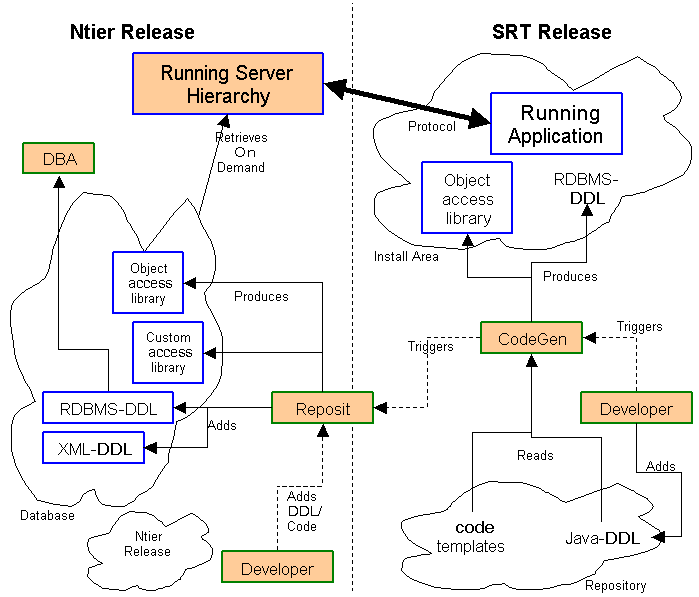
\includegraphics[width=\textwidth]{architecture.png}
\caption{Architecture of the \frontier system.\label{fig:architecture}}
\end{figure}

\section{Coupling}

Minimal logic in the client application.  Rules governing access to
objects/tables must be able to evolve independent of a client release.
Old clients must not prevent improvements or enhancements to newer
client applications.

\section{Protocol}

The protocol should allow prefetch algorithms in low-level servers to
add information that the server suspects you will be asking for in the
near future to current requests. If caching in middle layers of the
ntier system is down strictly on URL, this extra data may or may not
be present at some middle server. It may be a good idea to cause
cached URL expirations at a timely rate so that this newly added data
just appears like modified web pages.

It is possible to support general tabular data access in the
protocol. In other words, ntuple-like objects from database
tables. The result of such a query would include a description of the
data returned.

\subsection{Objects within a Server}

The server can be thought of as a collection of objects.  Each object has
a number of "get" methods that allow the user to ask for portions of data
within that object.  The arguments to the get methods are a set of keys.
The data returned is all the ``rows'' that match the set of keys.
Each object will have a type definition.  Users of this system must
supply type definitions or descriptions so that the server knows what
to deliver.  These definitions identify several important features:

\begin{enumerate}
\item the \emph{name} and \emph{version} of this type
\item the \emph{names} and \emph{types} of the attributes that will be
returned
\item the combinations of attributes that form \emph{keys}
\item an implied \emph{order} in which attributes are gaurenteed
to be delivered
\end{enumerate}

In addition to the things listed above, it may be worthwhile allowing
information that is domain specific, such as connecting this type
to a namespace or identifying SQL statements that can be used to
retrieve the information efficiently from a database.  Data type 
definitions will be in XML.

Below is the definition of the XML protocol which defines a single query
to a table or tables. 

\begin{verbatim}

<descriptor type="calibrunlist" version="1" xsdversion="1">
  <attribute position="1" type="int" field ="calib_run"/>
  <attribute position="3" type="float" field="calc_value"/>
  <attribute position="2" type="long" field="calib_version"/>
  <select>cr.calib_run, cr.calib_version, func(n)</select>
  <from>calibrunlist cr</from>
  <where>
    <clause>cid=@parm</clause>
    <param> position="1" type="int" key="cid"/>
  </where>
  <where>
    <clause>run=@param and xyz=@param</clause>
    <param position="1" type="int" key="run"/>
    <param position="2" type="string" key="xyz"/>
  </where>
  <final>order by ..... desc</final>
</descriptor>

\end{verbatim}

\begin{enumerate}
\item \emph{descriptor} - Top level tag describing what the data is for.
\begin{itemize}
\item \emph{type} - Name of the specific object this descriptor is for.
\item \emph{version} - Version number of the object.
\item \emph{xsdversion} - The version of XML servicer descriptor protocol which is being used 
to process the descriptor.
\end{itemize}
\item \emph{attribute} - Describles a datum which is being returned. The datum will be marshed 
according to the order of the \emph{attribute} tags.
\begin{itemize}
\item \emph{position} - The location of the datam in the \emph{select} tag this \emph{attribute}
is decribing.
\item \emph{type} - How the data will be marsheled out.  This is also the value returned when 
the client requests a description.  Valid values are:
\begin{itemize}
\item \emph{int}
\item \emph{long}
\item \emph{double}
\item \emph{float}
\item \emph{string}
\item \emph{bytes}
\item \emph{date}
\end{itemize}
\item \emph{field} - The name of the filed provided to the client when asked for a description.
\end{itemize}
\item \emph{select} - The fields returned from a query.
\item \emph{where} - A wrapper around tags which describe a specific where clause.  There may be 
multiples of this  tag.  The application decides on the \emph{where} to use based on the keys 
provided in the URL.
\item \emph{clause} - The SQL for the where clause, without the word ``where'', This will be used 
in the query.  Parameters may be passed in by useing the keyword ``@param''.  
\item \emph{param} - Identifies which ``@param'' keyword to replace with what value.
\begin{itemize}
\item \emph{position} - Which keyword to replace with this parameter
\item \emph{type} - How that keyword string is to be translated.  Valid values are
\begin{itemize}
\item \emph{int}
\item \emph{long}
\item \emph{double}
\item \emph{float}
\item \emph{string}
\item \emph{date}
\end{itemize}
\item \emph{key} - What key, supplied on the URL, which is being substituted into the parameter.
\end{itemize}
\item \emph{final} - Any final SQL clause which should be included in the query.  This tag may
be left empty or omitted.

\end{enumerate}

In this definition a single description contains one select.  That select may have multiple where
clauses.  The where clause is chosen based on the keys provided in the URL.  Consideration was given
to allowing multiple selects in a description.  This has not been included due to the amount of 
effort required versus the amount of expected use.  

Consideration was also given for adding a second descriptor which defines how to convert the data
from the result set to the user object.  This has been put off to keep the initial implemention
fairly straight forward.  It may be added in the future.  The tag \emph{xsdversion} was added to 
make these changes possible.


\subsection{Nature of the returned data}

The structure of returned data is tabular and
record-oriented, very much like a table in a relational database or that
of a spreadsheet.
A significant difference is that the \emph{atoms} of the row can include
arrays of both fixed and variable size of fundamental \cpp
types\footnote{``Fundamental types'' include all primitive types and
also strings.}.  The type definition describes a single row, the
returned data is a collection or sequence of these rows.

We imagine supporting three types of data representations:
\begin{enumerate}
\item BLOB
\item CSV
\item XML
\end{enumerate}

Example data used for the next sections:
\begin{verbatim}
struct Thing { int i; string s; short h[3] };
vector<Thing> v(2);  // <----- we want to receive this

// values as we want to see them in memory at the end
Thing* t = { {1, "scum", { 0x5555, 0x6666 } },
             {2, "swine",{ 0x7777 } }
           };
\end{verbatim}

\subsubsection{The BLOB}
Here are the rules regarding BLOB data.

\begin{enumerate}
\item allowed types are those available in C++ and arrays of them, this includes std::string
\item byte ordering is that of Intel - little endian
\item size of the allowed types are that of a 32-bit architecture machine.
\item arrays are always prefixed with the number of elements
\item all arrays are encoded as though they were variable length
\end{enumerate}

Because variable length arrays and strings are present, and because of
alignment issues in the stream, we cannot just use structure overlays
on the incomming data buffer.  Deserializers are necessary.  We can easily code
generate these functions.

Below is the byte stream we could except to see for our example data:

\begin{verbatim}
vvvviiiisssssssshhhhhhhhhhhhiiiissssssssshhhhhhhh
----|---|-------|-----------|---|--------|----------------------
000200010004scum00025555666600020005swine00017777
----|---|-------|-----------|---|--------|----------------------
\end{verbatim}

\subsubsection{The CSV}
The problem here is representing arrays at fields. 
\begin{verbatim}
1,"scum","0x5555,0x6666"
2,"swine","0x7777"
\end{verbatim}

\subsubsection{XML}
\begin{verbatim}
<row i="1" s="scum" h="0x5555,0x6666" />
<row i="2" s="swine" h="0x7777" />
\end{verbatim}

An alternative would be
\begin{verbatim}
<row><i>1</i><s>scum</s><h>0x5555 0x6666</h>
<row><i>2</i><s>swine</s><h>0x7777</h>
\end{verbatim}

As long as we have well-defined class definitions, mostly generated by
a program from some data definition language, we to not need to specify
the columns we want, or have the column information included in a 
response.

\subsection{Structure of Requests}

A request is encoded in a single URI\footnote{\textit{U}niversal
\textit{r}esource \textit{i}dentifier.} The details of format for a URI
is highly domain-specific; it may differ from experiment to experiment.
Multiple requests may be sent in the same URI.

The common pieces of information needed are:

\begin{enumerate}
\item the \emph{type} of data requested, and
\item the \emph{version} of that type.
\item a set of \emph{keys and values} specific to the type
\item an optional parameters indicating that results be
follow a specific \emph{data representation}
\end{enumerate}

Together these attributes identify a specific selection or instance
of a data object.  Each request within a URI must be fully described
before the next \emph(type) is encountered.

\subsubsection{Universal Query Concept}

\begin{verbatim}
 type=''string_name:version_number'' &
 encoding=BLOB|CVS|XML &
 key1=value1 & key2=value2 ...



where string_name:version_numer is the type name and its version number
appended into one string.  This forces them to ride together and
prevents conflict with other notioning of versioning that will be
present in the requests and results.

where encoding is required. It expresses what format we want the 
result in.  There is no default, it must be supplied for each request 
in the URI and may be different for each.

where key1,key2... are allowed keys to find data objects. Each of 
these keys would be specific to a type, such as CID for a calibration
type and DataRun for a CDF UsedSet query.
\end{verbatim}

There is an implicit or hidden parameter in this style request.
The request can be viewed as a method call.  The method name is
implicit in this request - it is always assumed to be RetrieveData.

This query works for locating class definitions and catalog information
as well as for the data itself.  If a definition of a type or class is viewed
as an instance of a type called "Description", then the instance could be
the name of the type.  Using the query for type information and 
by using the attributes argument, one can construct a generic browsing
tool or a tools that allows one to transfer the information into 
a statistical analysis tool such as R or into ROOT.

\subsubsection{Examples in the case of CDF}

\begin{verbatim}
type=SiChipPed:0 & CID=17443
 (here SiChipPed, version 0 is the object view of the table we want,
  17443 is a CID which identifies the specific instance we want,
  returned data is a BLOB containing
  all attributes of the table SiChipPed in the order described in 
  the SiChipPed type definition)

  <frontier version="1.9" xsdversion="1.3">
  <transaction payloads="1" crc="42427">
  <payload type="SiChipPed" version="0" CID="17443" encoding="BLOB">
  <data count="4">
  (see BLOB format for an example for the data returned)
  </data>	
  </payload>
  </transaction>
  <quality error="0"/>
  </frontier>

type=SiChipPed:0 & CID=17443 & encoding=CSV
 (here SiChipPed, version 0 identifies the type of thing we want,
  17443 is a CID instance ID, returned data is an CSV representation of
  all attributes of the table SiChipPed in the order described in the 
  type definition)

  <frontier version="1.9" xsdversion="1.3">
  <transaction payloads="1" crc="43847">
  <payload type="SiChipPed" version="0" CID="17442" encoding="CSV">
  <data count="4">
  1, 1.01, .04\\n
  2, 1.08, .05\\n
  3, 1.03, .04\\n
  4, 1.02, .06\\n
  </data>	
  </payload>
  </transaction>
  <quality error="0"/>
  </frontier>

type=Description:0 & encoding=XML & name=SiChipPed
  (get the description of the SiChipPed class in XML format)

  <frontier version="1.9" xsdversion="1.3">
  <transaction payloads="1" crc="5453">
  <payload type="SiChipPed" version="0" CID="17442" encoding="XML">
  <data count="1">
  <entry type=int name=CID />
  <entry type=int name=ChanID />
  <entry type=double name=Slope />
  <entry type=double name=Error />
  </data>	
  </payload>
  </transaction>
  <quality error="0"/>
  </frontier>

type=UsedSet:1 & process="CDF_PHYS_PROD" & run=144321 & version=3
  (get usedset entry for processname CDF_PHYS_PROD, datarun 144321, version 3)

type=CalibRunList:0 & table="SiChipPed" & run=4887 & version=4
  (get calibration data for calib run 4887, version 4, for sichipped)

\end{verbatim}

The full set of catalog queries are defined by the following classes
in SRT package CalibDB for CDF:

\begin{enumerate}
\item PASSES.hh, PASSCALIBS.hh (this is actually defined in DBViews)
\item UsedSet.hh
\item ValidSet.hh
\item RunList.hh
\end{enumerate}

There may be other objects that need to be supported from CalibDB.

\subsubsection{CDF Calibration Object Keys}

In regards to calibration data, CDF wishes to identify instance IDs
initially using a CID.  If we look closely at a CID, we will notice
that a single CID uniquely identifies both the type and instance of
the object requested.  We will not take advantage of this and assume
that type and CID are needed in a request.

In many cases, the programs know, in advance, a number of CIDs
that are needed.  It would be nice if a CID request could be
specifies as a range or set of values.  This case could make 
caching by URI alone difficult because of the variability in the
range or set specification amongst the programs.

CIDs are found by looking in a catalog (CALIBRUNLISTS) using more
interesting, human readable terms.  There are
several important ways to locate one or more CIDs:

\begin{enumerate}
\item By \emph{Calibration run number} or \emph{run range},
or a list of run numbers.
\item By \emph{Data run number} or \emph{run range},
or a list of run numbers.
\item By production \emph{Pass number} or list of pass numbers.
\end{enumerate}

We will assume that it is necessary to first go to a catalog table to
to locate the desired CID, and then execute a separate query to retrieve
the data.

Each specified \emph{type} of data must have a specified \emph{version}
attached to it. The term version is used in several different contexts at
CDF.  This use purtains specifically to a schema version or object
definition version.

\subsection{Structure of a Reply}

The examples above already illustrated the data portion or payload of a reply.
A reply consists of \emph{metadata} describing the enclosed
\emph{data payload(s)}.
A reply will consist of a sequence of zero or more individual payloads.
Different types or instances of data objects are never coalesced into a single
payload bundle; they are received as distinct items.

The reply is an XML datagram.  The XML serves as a descriptive wrapper
around the data payload.

The datagram XML's protocol identifies the data being returned, detailing the contents 
of each section of data being returned being quality of the data section. An example of a 
datagram is provided below and a description of each tag follows. The indentation is provided, only
for readability of this document and will next exist in the production version.

\begin{verbatim}
<frontier version="1.9" xsdversion="1.3">
  <transaction payloads="2">
    <payload type="thing1" version="1" encoding="blob">
      <data>
        yada yada yada yada yada yada yada yada yada
      </data>
     <quality records=3 error=1 code="666" message="Trust me its bad!"/>
    </payload>
    <payload type="thing2" version="1" encoding="blob">
      <data>
        yada yada yada yada yada yada yada yada yada....
      </data>
      <quality records=17 error=0"/>
    </payload>
  </transaction>
  <quality error="0"/>
</frontier>
\end{verbatim}

\begin{enumerate}
\item \emph{frontier} - Provides identifying data about the product.
\begin{itemize}
\item \emph{version} - Current version of the product.
\item \emph{xsdversion} - Current version of the XML protocol in use.
\end{itemize}
\item \emph{transaction} - General wrapper around data being returned.
\begin{itemize}
\item \emph{payloads} - A count of the payloads that are being returned.
\end {itemize} 
\item \emph{payload} - Identifies the specific data being returned for single
universal query.
\begin{itemize}
\item \emph{type}- The object being returned.
\item \emph{version} - The version of the object being returned.
\item \emph{encoding} - The method by which this data was encoded.
\end {itemize}
\item \emph{data} - Encloses the actual data being returned to the client.
\item \emph{quality} - Identifies any errors encounted in producing the data, including sytax errors.
\begin{itemize}
\item \emph{records} - Number of tuples in the data.
\item \emph{error} - 0 if no error occurred else 1. 
\item \emph{code} - Integer code of the error. Only provided if error occurred.
\item \emph{message} - Text message related to the error code. Only provided if error occurred.
\end {itemize}
\end{enumerate}

The ending \emph{quality}'s \emph{error} is set to 1 if a syntax error occurred in first level parsing of the URL.  

\subsubsection{Data}


The data is binary encoded, in \spec{Base64} format.
\begin{fixme}
Put a reference for the definition of Base64 here.
\end{fixme}

\subsection{Error Handling}


\section{Versioning}

We imagine having several entities which are types, such as a table in
a database and a class that holds the information from the table. Over
time, the definition of the type can change. How is this change
manifested? Can table type definitions be modified without a name
change or does modification imply just a new version? Can old and new
clients have class names that are the same but with different versions
on the request so the server knows how to fill them properly? 

There are many problems assocaiated with the generation and recording
of version numbers.  The version number plus the class name really 
identify a unique type.  The versioning method must work well
for releases as well as for developer using private releases. 
Here are three techniques that can be used to
manage this type information.

\begin{enumerate}

\item Global Registry
\item GUID or hash code
\item User assigned.

\end{enumerate}


The global registry is a centralized database that stores all type 
definitions and generates version numbers for them.  A user of the
system must submit the type definition to this facility and then
receive out a version number for it.  This means that each build
that actually runs the ``codegen'' step for table access must submit
a request to a server.

The idea behind the GUID is that a object is generated and tagged
with a ``global unique identifier''.  This value determines where
this object lives.  In the case of our table definitions, this
object type would be of type ``Class''.  The problem here is that
contacting that object requires distributed processing machinery
such as nameservers and perhaps a global object repository.  Using
a GUID or something similar as just a hash code that encodes the 
name and attributes is interesting. The problem is that hash codes
are not gauranteed unique.  You can only really tell if two things
are not the same.

Allowing the user to assign the version number himself is easy.
The problem here is that the user must know how, when, and where
to do it.  In terms of CDF, we have a place for it in the
data definition java file.

The ntier system separates experiment code builds and releases from 
ntier builds and releases.  Where do the type definitions live?
The diagram shows the main source of definitions in the experiment
code repository and being pushed to the ntier system during 
the build system's ``code generation'' phase.  This implies that
there exists some king of global repository of definitions within
the ntier domain.  From the requirements, we have some constraints
placed upon us: Developers must be able to play - generate new 
defintions, attach to development database to test iteratively.
This means that we need to have several instances of a ntier
system running to service the different types of users (developers,
production, and perhaps testers and others). 
\emph{The build environment will need to know which one to correct for the user}.

Here is a proposal for managing definitions and versions.  Version
numbers are incremented and assigned by the experiment.  At CDF,
this is in the java DDL file.  The ntier project will publish a 
format that it wants to receive new DDL files in.  The build system
will be assigned to an ntier instance.  That ntier instance will
maintain a repository of type definitions.  The build system will
submit the DDL to the ntier instance.  The ntier instance will 
generate a hash code (using MD5 or CRC) using the definition file
information and first check to see if the definition already exists.
The definition will be added to the repository or verified during the
submission process.

\section{Client Functions}

\begin{fixme}
What is the client allowed to do? What is its role in the system?
\end{fixme}

\section{Server Functions}

\begin{fixme}
What is the job of the servers?
\end{fixme}

\section{Monitoring and Control}

\begin{fixme}
What are the monitoring and control paths for the client and server?
Are they the same or different than the main data path? Is the
protocol different?
\end{fixme}



\section{Code Generation}

\begin{fixme}
Does code generation take place for the server? What is its
relationship with the client generated code? Why and when is it
necessary? When is it not necessary?

It is possible to generate definitions and even libraries directly
into a database that is accessible by every low-level server. Such a
situation would allow demand loading of new definitions and code by
servers as unknown objects are requested by clients.

\end{fixme}


\section{System Configuration}

\begin{fixme}
What parts of the system must have fixed configuration? What
parameters are dynamic? What is tied to a release and what is not?


We want to system to support incremental adding of new table/object
mapping libraries to running servers. The rules are that currently we
will support adding new code to running servers. To install a new
version of existing libraries or to remove a library will require
reloading or restarting a servlet or running component.

We need to add information about the global distribution function
here. It needs to support attaching to a development set of
servers. It needs to support authentication of users to allow plain
old developers to distribute code continuously to development servers
and also to remove it, send changes, and reset servlets.

How are DDL files propagated to DBAs or managers?  How are table and
object versions managed in a development setting as opposed to a
production setting?

We need to further define the ntier release type definition repository
and the format of a definition.  How the experiment build system
contacts this repository to ship definitions to is another issue
that needs to be completed.  As stated above, we may want to declare
some ntier systems as capable of receiving object definitions to
store and distribute to other tier-0 servers.  examples of named
ntier systems are development, production, and test.
\end{fixme}

\section{Release Management}

\begin{fixme}
How are releases of the \frontier project handled and how are they
related to releases of the experiments' client code? How much of the
\frontier code is experiment-specific, and how are releases of that
code synchronized with the experiment's code? How much can the
\frontier core code schedule be decoupled from that of any and all
experiments using \frontier?
\end{fixme}

Code management in \frontier is handled in two distinct parts. Code
that is part of the core of \frontier is managed centrally by the
\frontier development team (eventually to be handed over to a
\frontier maintenance team). Code that is used by \frontier but that
is specific to the needs of a specific experiment (or other client) is
developed in concert with the \frontier development team, and
maintained by the experiment (or other client).

\begin{figure}[hbt]
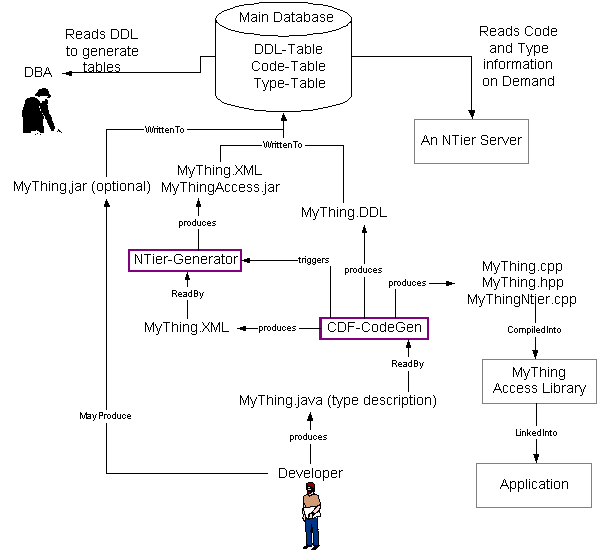
\includegraphics[width=\textwidth]{adding_defs.png}
\caption{Architecture of the \frontier system.
\label{fig:development}}
\end{figure}

The \ref{fig:development} figure shows the flow of information when
a developer adds a new type definition into the system. Developers
attach a release to a specific ntier/database instance.  If the
developer is creating and trying out new definitions, he may be
attached to the development database and ntier instance.  If he
is doing work out of a production release, that release may be
attached to the production database and ntier instance.

Developers are expected to create table/object definitions as they
do today.  In the case of CDF, this mean java-DDL and the CDF code
generation system.  The code generator will need to produce a 
type definition that the ntier system expects in addition to the 
RDBMS-DDL that it already generates.  The build system will need to
run a utility contained in the ntier release that performs the upload
of this ntier type definition into the database.

Developers will have the option of choosing the generic ntier access
generation or to create a custom access library.  For simple data tables
(as in the calibration tables at CDF now), a one-to-one mapping between
object and table may be adequate.  In this case, the developer can choose
to have the ntier access library generated automatically.  If the
new object complicated, such as a view across several tables, then the
developer can supply a custom access library that will map the set of
tables to the desired type.

Here is a summary of some of the important properties of this system:
\begin{enumerate}
\item it allows for more than one instance of the ntier system, each
of which is attached to a set of databases
\item all type definitions and table definitions go into the database
\item DBAs or other priviledged individuals pull DDL out of the database
to generate new tables.
\item The ntier servers retrieve new definitions and code from the database
when they receive requests for types that they know nothing about
\item developers can supply custom access code or choose to have 
the simple generic generated for them.
\end{enumerate}










\chapter{Technology}

\section{Overview}

\begin{fixme}
This entire section is notes---not final text.
\end{fixme}

The internet is filled with widely accepted, production quality,
frameworks and tools used for delivering database, and other
information using the HTTP protocol.There are several general
technologies used for serving dynamic content pages including Tux,
Apache, PHP, Perl, Python, and Server-Side Java. Database access and
pool management for the database connections has been developed for
many of the server products as well, we know that we will need to
access oth Oracle, MySQL, and possibly other database
platforms. Caching of dynamic content pages is not normal, but it is
possible to build it into the server products, and also there are many
caching proxy server products which offer reasonable performance and
versitile configuration options to meet our needs.  In addition,
whatever products are deployed the server performance monitored. Some
of the products reviewed have monitoring features built in, and some
do not. There are many tools available for watching the overall
performance of machines running the servers such as memory, cpu, and
netword activity.

{reference L. Titchkosky, M. Arlitt, C. Williamson, ``A Performance
Comparison of Dynamic Web Technology,'' Performance Evaluation Review,
volume 31 number 3, December 2003, pp2-11.}

There is a broad array of server software approaches used on the
internet to deliver dynamic content pages including Tux, Apache, PHP,
Server-sise Java, Perl and python.

{reference
http://www.redhat.com/docs/manuals/tux/TUX-2.2-Manual/intro.html} Tux,
also known as Red Hat Content Accelerator, is a high performance
kernal-based web server for Linux. Red Hat Content Accelerator runs
partly within a custom version of kernel 2.4.x or higher and partly as
a user-space daemon. With a capable network card, Red Hat Content
Accelerator enables direct scatter-gather DMA from the page cache
directly to the network, thus avoiding data copies. Whenever Red Hat
Content Accelerator is unsure how to process a request or receives a
request it is unable to handle, it always redirects the request to the
user-space web server daemon to handle it in an RFC-compliant
manner. An example of this user-space web server daemon is Apache.It
is currently limited to serving static webpages and coordinating with
kernel-space modules, user-space modules, and regular user-space Web
server daemons to provide dynamic content. Regular user-space Web
servers do not need to be altered in any way for Red Hat Content
Accelerator to coordinate with them. However, user-space code has to
use a new interface based on the tux(2) system call. Red Hat Content
Accelerator also has the ability to cache dynamic content. Red Hat
Content Accelerator modules (which can be build in kernel space or in
user space; user space is recommended) can create "objects" which are
stored using the page cache. To respond to a request for dynamic data,
a Red Hat Content Accelerator module can send a mix of
dynamically-generated data and cached pre-generated objects, taking
maximal advantage of Red Hat Content Accelerator's zero-copy
architecture.


Apache can be used to serve dynamic content pages by including plugins
which are available for many languages including PHP, perl, python,
and Java. It has the advantage that most of the worlds web servers run
Apache, and it is well documented, highly configurable, and there are
many monitoring packages available for it.  PHP is a scripting
language specifically designed for the Web, and it is generally used
as a plug-in wiht Apache.

There are a number of Java products which provide server-side dynamic
content processing using modules, servlets, written in Java. Tomcat is
a servlet container that provides the official reference
implementation for both Java Servlets and Java Server
Pages. (http://jakarta.apache.org/tomcat) Jetty ia a Web server and
Java Servlet container written in Java. It is advertized as one of the
fastest servlet servers available. (http://jetty.mortbay.org/jetty)
Resin is a commercial Web server and Java servlet container freely
available to non-commercial users.

\hyphenation{language update}

\begin{table}[h]
\centering
\caption{What is this table about?}
\begin{tabularx}{\textwidth}{XXXXXX}\toprule
Product  & Performance & Configurability & Servlet Language & Servlet Update & Caching and Proxy Servers \\ \midrule
         &             &                 &                  &                &                            \\ \bottomrule
\end{tabularx}
\end{table}

\section{Caching and Proxy servers}

Caching is configurable for, or can be built into, many of the servers
discussed above. Another approach which can be used in conjunction
with the dynamic content servers is an independent layer of caching
provided by proxy servers. For a comprehensive overview of this
technology see (Duane Wessels, Web Caching) This is a well understood
technology used on the internet to provide performance and reliability
across the internet, although it is rarely used in conjunction with
dynamic content pages. Proxy caching servers provide many features
which make them attractive including authentication, request
filtering, response filtering, prefetching, translation and
transcoding, and traffic shaping. They can be interconnected in
various configurations of meshes, clusters, hierarchies.

There are many products available which are interesting for our
use. Squid is an open source package that runs on a wide range of unix
platforms and it is highly configurable. Netscape Proxy Server runs
oon unix systems as well and windoew NT, and is one of the first proxy
products. CacheFlow provides intellegent prefetching and refreshing
features. InfoLiberanis designed for reliability and fault
tolerance. There are several other products which can be purchased or
run on proprietary hardware.

Caching proxies provide the ability to configure the cache management
and cache sharing among groupings of servers. Cache management can be
controlled with several policies, like LRU. A variety of inter cache
protocols are available inclueing Internet Cache Protocal (ICP), Cache
Array Routing Protocal (CARP), Hypertext Caching Protocol (HTCP), and
Cache Digests.

System performance and reliability need to be planned and there are
several approaches to load balancing and fail over that can be
considered, if expensive hardware is not an option. High availability
systems can be built with, UPS, dual redundant power supplies,
processors, et cetera, and raid disks. Alternatively, some simple DNS
tricks and complex load balancing. Layer foru switches can be
configured to intellegently manage failure detection as well.  Load
sharing techniques include DNS round Robin, Layer four switches, CARP,
ICP.

Because of the popularity of this technology, there are numerous
monitoring tools availabel as well. Some Proxy Caching servers provide
SNMP interfaces for which there are numerous analysis and charting
utilities available. Also, log analysers are availale for logs
formatted in ``standard'' formats, which most PCS's provide. Commonly
used monitoring tools such as MRTG and RRDTool enable easy access to
the performance data coming from each server.

In additon to monitoring the software server itself, it is generally
useful to monitor machine performance. Tools such as Ganglia, nagios,
and tcpdump provide convenient solutions for monitoring distributed
systems.

Sun provides the base classes for JDBC, on which third party database
venders layer their specific implementations. Oracle and MySQL supply
jar files with their particular derived subclasses.

Some vendor database connections are lab wide limited by license. We
therefore consider database connections to be a critical resource
which must be monitored.  A pool of available database connections
will be provided.  This pool will be configurable as to the maximum
and minimum number of connections allowed and how long an idle
connection may remain open.  Server connection requests will be filled
from and returend to this pool.  Any available connection will be
given to the request.  If none is available a new connection will be
created up to the maximum pool size.  After that requests will be
queued until an existing connection is returned to the pool.

We belive it is possible to supply a connection pool with third party
software such as the DbConnectionBroker provided by JavaExchange.com
or the connection pool which comes with Tomcat.

Need to figure out JNDI

Discussion of the commercial products goes here: Java, servlets,
MySQL, JDBC, squid, ganglia, nagios, tcpdump, cURL, nameservice,
redundancy, \etc%Note that 'etc' carries a period already.


\section{Choices}

\begin{fixme}
What goes here?
\end{fixme}



\chapter{Analysis and Design}

\section{Protocol}

Here we place a concrete proposal for the communication protocol
between client and server.

\section{Client}

The design of the client API library and interactions with the code
generator.

\section{Server Translation}

Here we discuss how a server maps from the information in a database
table to an object that the user requested.

\section{Monitoring}

Here is a listing of the things we want to monitor in the system and
how that data will get to collection points.
\section{Utilities and Tools}

\begin{fixme}
Here we discuss the tools that are needed to satisfy remote
administration requirements.
\end{fixme}


\chapter{Development Approach}

\begin{fixme}
Here we discuss the incremental approach we are using to develop this
product. The basic idea is that we make small steps forward in
technology and complexity and test and evaluate them to make sure we
are moving in the right direction. The steps turn into a series of
experiments.
\end{fixme}

\section{Experiment Monitoring---Capture and Reporting}

The data recorded from a test or experiment must be captured and
tagged in a global place so that everyone can analyze it.

\begin{fixme}
More is needed here.
\end{fixme}

\section{Experimental Environment}

\begin{fixme}
What machines or configuration is needed to run the tests and
experiments we need to run?
\end{fixme}

\section{Experiment Sequence}

\begin{fixme}
Here we discuss a potential series of tests or experiment that will
address the questions of whether or not the system will perform as
expected.
\end{fixme}

\section{Possible Configurations}

\begin{fixme}
What are some of the ways we to configure products like squid? We want
to determine the set of configurations that we will promote and
support.
\end{fixme}


\chapter{Release Management and Testing}

\begin{fixme}
A concrete proposal for managing ntier releases and automated testing
goes here.
\end{fixme}


\chapter{Deployment}

\begin{fixme}
A plan for deployment and support goes here. Include hardware
requirements (networking, memory, CPU).
\end{fixme}


% ----------------------------------------------------------------------
%\begin{thebibliography}
%\end{thebibliography}
% ----------------------------------------------------------------------
\end{document}
